\documentclass{amsbook}
\usepackage{graphicx} % Required for inserting images
\usepackage{float}
\usepackage[colorlinks=true,linkcolor=blue]{hyperref}
\usepackage{amssymb}
\usepackage{enumerate}
\usepackage{mathtools}
\usepackage{tikz}
\usepackage[answerdelayed]{exercise}
\usepackage{floatflt}
\usepackage{multicol}
\usepackage{subcaption}
\usepackage{tikz}
\usepackage{tkz-euclide}
\usetikzlibrary{trees}
\usepackage[backend=biber,style=alphabetic,sorting=ynt]{biblatex}
\addbibresource{calc.bib}

\setlength{\parindent}{0pt}
\setlength{\listparindent}{0pt}
\renewcommand{\ExerciseHeaderTitle}{\quad\ExerciseTitle}
\renewcommand{\AnswerHeader}{\medskip\centerline{\emph{\ExerciseName\ \ExerciseHeaderNB} \smallskip}}
\renewcommand{\ExerciseHeader}{\medskip\ExerciseHeaderDifficulty{\emph{\ExerciseName\ \ExerciseHeaderNB\ExerciseHeaderTitle} \newline}}
\renewcommand{\QuestionNB}{(\alph{Question})\ }
\renewcommand{\Re}{\operatorname{Re}}
\renewcommand{\Im}{\operatorname{Im}}

\begin{document}

\title{Calculus Problem Book:\\
    \Large Form V and Form VI}


\author{S. Chu}

\maketitle
\tableofcontents
\chapter*{Preface}
The following short booklet contains a collection of problems with solutions that roughly follow the topics typically covered in the calculus sequence for Form V and Form VI mathematics classes at Ethical Culture Fieldston School. The hope is to provide a book of problems of varying difficulty that will provide non-routine exercises as well as to record general themes and approaches to tackling these types of problems in general. Ideally these problems can be useful to all courses that cover these topics. Problems are roughly categorized by difficulty level and notated via *, **, or *** in increasing difficulty. We have adopted problems from memory, and from years of working with the material. The following references were consulted for problems as well as other considerations such as narrative structure in introducing various topics and thematic development of the material. \cite{mcirc}, \cite{aops}, \cite{hpn}, [more later].
\chapter{Functions and Other Miscellaneous Content}

\section{Number Systems}
\begin{Exercise}[title={Sets and Types of Numbers}, difficulty = 0, label= 1b1]
	Set $A \subset B$ iff every element of $A$ in also in $B$. Set $A \supset B$ iff every element of $B$ is also in $A$ and two sets are equal iff both $A\supset B$ and $A\subset B$.
	
\end{Exercise}


\section{Working with Inequalities}


\section{Polynomials}


%%

\begin{Exercise}[title={Polynomials I}, difficulty=0 , label=1a1 ]
	Let $f(x)=x^2-3$ and $g(x)=x^3-2x$. Both $f$ and $g$ are polynomials. You can form new polynomials by adding, subtracting, multiplying, and composing. 
        \begin{enumerate}
            \item Find $(f+g)(x)$
            \item Find $(f-2g)(x)$
            \item Find $(f\cdot g)(x)$
            \item Find $f \circ g)(x)$
            \item Explain why $(f/g)(x)$ is not a polynomial.
        \end{enumerate}

	\hfill \emph{solution} \refAnswer{1a1}
\end{Exercise}

\begin{Answer}[ref={1a1}]
	blah blah
\end{Answer}

\begin{Exercise}[title={Defining Polynomials}, difficulty=1, label=1a2]
A polynomial $f$ has the general form $f(x)=a_0+a_1 x + a_2 x^2 + \ldots +a_{n-1}x^{n-1} + a_nx^n$, where $n \in \mathbb{Z}$ and $a_i \in \mathbb{R}$. Show that adding, subtracting, or multiplying two polynomials always results in a polynomial. Explain why this is not the case for division.

    \hfill \emph{solution} \refAnswer{1a2}
\end{Exercise}

\begin{Answer}[ref={1a2}]
    The expression $A \subset B$ is read, the set $A$ is contained in the set $B$. Whereas the expression $A \supset B$ is read the set $A$ contains the set $B$.
    \begin{enumerate}
        \item $\mathbb{Z}\supset \mathbb{N}$
        \item $\mathbb{R}\supset \mathbb{Q}$
        \item $\mathbb{N} \subset \mathbb{Q}$
    \end{enumerate}
\end{Answer}

\begin{Exercise}[title={Polynomials II}, difficulty =0, label=1a3]
   A function $f$ is even if and only if $f(x)=f(-x)$ for all $x$ in its domain. A function is odd if and only if $f(-x)= - f(x)$ for all $x$ in its domain.
   	\begin{enumerate}
   		\item Give an example of an even polynomial.
   		\item Give an example of an odd polynomial.
   	\end{enumerate}
\end{Exercise}

%%%%%%%%%%%%%%%%%%%%%%%%%%%%%%%%%%%%%%%%


\section{Trigonometric Functions}

%%%%%%

\section{Miscellaneous}

%%%%%%%%%%%%%%%%%%
%%%%%%%%%%%%%%%%%%
\chapter{Limits and Continuity}


\section{Intuitive Notion}

\section{Epsilon and Delta}

\begin{Exercise}[title={Dirichlet Function}, difficulty=1 , label=2b1 ]
	The Dirichlet function $D$ is define as $D(x)=\left\{\begin{array}{c l} 1 & x\in \mathbb{Q} \\ 0 & \mbox{otherwise}\end{array} \right.$. Two sets of numbers are \emph{not seperable} if it is impossible to find an open interval around an element from one set that contains only elements from that set and not the other. Rational numbers and irrational numbers are not separable. Use this  to argue that $\lim \limits_{x\to a} D(x)$ does not exist for any value of $a$.
	\hfill \emph{solution} \refAnswer{2b1}
\end{Exercise}

\begin{Answer}[ref={2c1}]
	blah blah
\end{Answer}
\section{Continuity}
\begin{Exercise}[title={A Bounded Function around Zero}, difficulty=1 , label=2c1 ]
	Let $f: \mathbb{R} \to \mathbb{R}$ be a function such that $|f(x)| \leq |x| $ for all $x$ in the domain of $f$.  Prove that $f$ is continuous at $x=0$.

	\hfill \emph{solution} \refAnswer{2c1}
\end{Exercise}

\begin{Answer}[ref={2c1}]
	blah blah
\end{Answer}

\begin{Exercise}[title={Some Points Don't Move That Much}, difficulty=1 , label=2c2 ]
	Let $f:[0,1] \to [0,1]$ be a function such that $|f(x)| \leq |x| $ for all $x$ in the domain of $f$.  Prove that $f$ is continuous at $x=0$.

	\hfill \emph{solution} \refAnswer{2c2}
\end{Exercise}

\begin{Answer}[ref={2c2}]
	blah blah
\end{Answer}


\section{Intermediate Value Theorem}


%%%%%%%%%%%
%%%%%%%%%%5

\chapter{The Derivative}

\section{Limit Definition and Properties of the Derivative}
\begin{Exercise}[title={Introducing a Discontinuity}, difficulty=0, label=3a1]
Let $f(x)=|x|$. Use the limit definition of the derivative to show that $f'(x)=\dfrac{|x|}{x}$. Show using the definition of continuity how the derivative 

\end{Exercise}

\begin{Answer}[ref={3a1}]
    
\end{Answer}

\section{Tangent Line Problem}

\section{Higher Order Derivatives}

\section{Power Rule and others}
\begin{Exercise}[title={Unit Circle and Sine}, difficulty=1 , label= 3d1]
	Let $P=(\cos \theta,\sin \theta)$. Use similar triangles to calculate an approximation for $\dfrac{\Delta y}{\Delta \theta}$ and explain how this shows what the derivative of $f(x)=\sin (x)$ is.  Do the same for $g(x)=\cos(x)$ by looking at $\dfrac{\Delta x}{\Delta \theta}$.
		\begin{figure}[H]
			\centering
			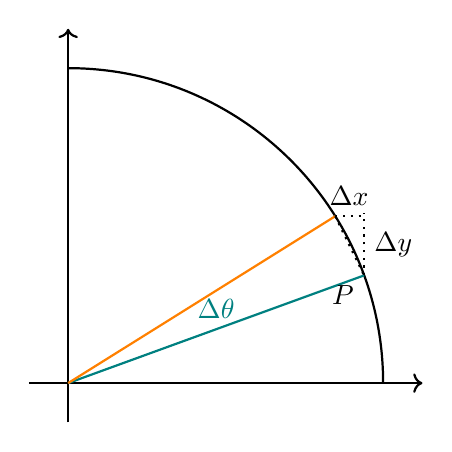
\begin{tikzpicture}
			\draw[thick](4,0)arc(0:90:4);
			\draw[thick,->](-.5,0)--(4.5,0);
			\draw[thick,->](0,-.5)--(0,4.5);
			\tkzDefPoint(4,0){A}
			\tkzDefPoint(0,0){B}
			\tkzDefPointBy[rotation=center B angle 20](A) \tkzGetPoint{C}
			\draw[thick, color=teal](B)--(C) node[midway, above]{$\Delta \theta$};
			\tkzDefPointBy[rotation=center B angle 12](C) \tkzGetPoint{D}
			\draw[thick, color= orange](B)--(D);
			\draw[thick,dotted](C)--+(0,.79) node[midway,right]{$\Delta y$};
			\draw[thick,dotted](D)--+(.35,0) node[midway, above]{$\Delta x$};
			\draw[thick,dotted](D)--(C) node[at end, below left]{$P$};
			\end{tikzpicture}
		\end{figure}

	\hfill \emph{solution} \refAnswer{3d1}
\end{Exercise}

\begin{Answer}[ref={3d1}]
	blah blah
\end{Answer}

\section{Implicit Differentiation}

%%%%%%%%%%
%%%%%%%%%%%

\chapter{Applications of the Derivative}

\section{Related Rates}

\section{Mean Value Theorem}

\section{Maximums and Minimums}

\section{Optimization and Graphing}

%%%%%%%%%
%%%%%%%%%

\chapter{The Integral}
\section{Series}

\section{Riemann Sums}

\section{Riemann Integrable}

\section{Properties of the Integral}

%%%%%%%%%%%
%%%%%%%%%%%%

\chapter{The Fundamental Theorem of Calculus}
\section{Anti-Derivatives}

\section{FTC part I}

\section{FTC part 2}

\section{Functions Defined by an Integral}

\section{Integral as Accumulator}

\section{Probabilty Distributions}

%%%%%%%%%%%%
%%%%%%%%%%%

\chapter{Logarithms and Exponentials}

%%%%%%%%%%
%%%%%%%%%%%%

\chapter{Methods of Integration}
\section{U Substitution}

\section{Integration by Parts}

\section{Method of Partial Fractions}

\section{Trigonometric Substitutions}

\section{Improper Integrals}

%%%%%%%%%
%%%%%%%%%

\chapter{Differential Equations}

%%%%%%%%%%
%%%%%%%%%%

\chapter{Applications of Integration}

%%%%%%%%%%
%%%%%%%%%%

\chapter{Infinite Series}

\chapter{Conics, Parametric Equations, Polar Coordinates}

\chapter{Vectors and the Geometry of $\mathbb{R}^3$}

\chapter{Vector Valued Functions}

\chapter{The Partial Derivative and Function of Several Variables}

\chapter{The Gradient and the Method of Lagrange Multipliers}

\chapter{The Derivative of maps from $\mathbb{R}^n \to \mathbb{R}^m$}

\chapter{Longer Problem Sets}
    \section*{Working with Parameters and the Derivative}
    	In this exploration we will work with derivative to find tangent lines to a curve. We will also introduce working with parameters and see how this gives us a set of tools to solve more complex problems. We will end by using our skill with parameters to explore a little bit of the early history of Calculus by taking a look at Descartes' Method of Normals and Fermat's Method of Adequality.
    	\subsection*{First Let's Look at Tangent Lines to a Parabola}
    		\begin{enumerate}
    			\item Let $f(x)=x^2+1$ and point $C(0,-2)$. Find the equation of the two lines that pass through $C$ and are tangent to $f$.\\
    			
				\item Let $C$ vary its position along the $y$-axis. Let $C(0,k)$. Find the equations of the two lines that pass through $C$ and are tangent to $f$. Notice your solutions will be in terms of the 				parameter $k$.\\
				
				\item Lastly, let's generalize and let $C$ be any point in the plane $C(h,k)$. What are the equations of the two lines that pass through $C$ and are tangent to $f$, in terms of the parameters $h$ and $k$? \\
				\item Notice this gives you the equations for the lines through any point in the plane that are tangent to the given parabola. Demonstrate the ease with which you can find these lines that are tangent to the parabola, by find them for $P(5,3)$ and $Q(3,-5)$.\\
				\item What do these equations tell you about the family of lines tangent to $f$? How is this different than just looking at $f'(x)$?\\
    		\end{enumerate}
    		
    	\subsection*{Descartes' Method Of Normals}
    		
    \newpage		
    \section{An Algorithm to Find Roots}
    
    \section{Efficient Foraging}
    
    \section{When is Venus Bright in the Sky?}
    
    \section{Rainbows}
    
    \section{Constructing the Demand Curve}
    
    \section{The Shape of Bee Hive Cells}
    
    \section{The Art Gallery Problem}
    
    \section{Getting to $\pi$ using Integration by Parts}
    
    \section{Predicting Peak Oil}
    
    \section{SIR: A Model for the Spread of Infectious Disease}
    
    \section{Modeling Air Resistance}
    
    \section{A Model for Combat}
    
    \section{A Model for Relationships}
    

%%%%%
%%%%%
%End of problems of the book.
%%%%%%%
%%%%%

\chapter{Answers}
\shipoutAnswer

\printbibliography
\end{document}
